\documentclass[12pt,a4paper]{article}
\usepackage{classeRapport} % template INSA
\usepackage{hyperref} % lien tableofcontents + url
\usepackage{graphicx} % pour les images
\usepackage{listings} % pour mettre du code
\usepackage{color} % pour la couleur dans le code
\usepackage{amsmath} % pour les matrices
\usepackage{float} % pour le [H] des figures
\usepackage{tikz} % pour tracer des figures
\usepackage{amssymb} % pour utiliser \mathbb{Z} : symboles entiers relatifs

\hypersetup{ % couleur des liens
    colorlinks=true,
    linkcolor=black,
    filecolor=black,      
    urlcolor=blue,
}

\definecolor{backcolour}{rgb}{0.95,0.95,0.92}
 
%%%%
\definecolor{mygreen}{RGB}{28,172,0} % color values Red, Green, Blue
\definecolor{mylilas}{RGB}{170,55,241}

\lstdefinestyle{mystyle}{
    backgroundcolor=\color{backcolour},   
    basicstyle=\footnotesize,
    breakatwhitespace=false,         
    breaklines=true,                 
    captionpos=b,                    
    keepspaces=true,                 
    numbers=left,                    
    showspaces=false,                
    showstringspaces=false,
    showtabs=false,                  
    tabsize=2,
    %%%%
    language=Matlab,
    morekeywords={matlab2tikz},
    keywordstyle=\color{blue},
    morekeywords=[2]{1}, keywordstyle=[2]{\color{black}},
    identifierstyle=\color{black},
    stringstyle=\color{mylilas},
    commentstyle=\color{mygreen},
    showstringspaces=false, % without this there will be a symbol in the places where there is a space
    numberstyle={\tiny \color{black}}, % size of the numbers
    numbersep=9pt, % this defines how far the numbers are from the text
    emph=[1]{for,end,break},emphstyle=[1]\color{red}, % some words to emphasise
}

\lstset{style=mystyle}

\begin{document}

\PageDeGarde
{Images/TemplateINSA/rien} % image sur la page de garde
{Canny-Deriche\\ Détecteur de Contours} % titre principal
{Projet TIM} % sous-titre
{Mehdi \textsc{ABOUZAID}\\
 Damien \textsc{TOOMEY}\\
 --\\
 À l'attention de \\ M. \textsc{Bensrhair}} % nom
{TIM - ASI - 2018-2019} % bas de page

\Page{INSALogo}{rien.png} % logo de bas de page (en bas a droite)

\newpage
\tableofcontents

\newpage
\section{Introduction}
L'intérêt majeur de la détection de contours est la réduction d'information. En effet, l'information d'une image peut être résumée par les contours des différents objets qu'elle contient car les contours contiennent les parties les plus informatives de l'image.

Pour certaines applications (reconnaissance de formes, imagerie médicale, cartographie,...), les contours de l'image suffisent pour l'exploiter. La détection de contours permet ainsi d'éviter de stocker des informations lourdes inutilement.

Dans ce rapport, nous allons nous intéresser au détecteur de contours de Canny-Deriche. \\

Le filtre de Deriche est un opérateur de détection de contours développé par Rachid Deriche en 1987. C'est un algorithme permettant la détection de contours dans une image à deux dimensions. Cet algorithme est une évolution du filtre de Canny développé par John Canny en 1986. 


\newpage
\section{Description du filtre}
\subsection{Etapes de la détection de contours}

Comme le détecteur de contours de Canny, celui de Deriche s'effectue en quatre étapes :

\begin{itemize}
	\item[\textbf{1}] Gradients et lissage (réduction du bruit)
	\item[\textbf{2}] Norme du gradient et direction du gradient
	\item[\textbf{3}] Suppression des non-maxima locaux
	\item[\textbf{4}] Seuillage par hystérésis
\end{itemize}

\subsection{Critères du filtre}

	Dans le filtre de Deriche, on retrouve les mêmes critères de détection optimale des contours du filtre de Canny : 	
\begin{itemize}
	\item[\textbf{A}] Bonne détection : faible taux d'erreur dans la signalisation des contours. Il ne faut manquer aucun contour, ni en rajouter (faux positifs)
	\item[\textbf{B}] Bonne localisation : les points détectés comme contours doivent être aussi proches que possible des points de contours réels
	\item[\textbf{C}] Clarté de la réponse : un point du contour ne doit être détecté qu'une seule fois par le filtre. Ce critère est inclus implicitement dans le premier critère puisque si l'on détecte deux contours là où il n'y en a qu'un, une des deux réponses doit être considérée comme fausse. \\
\end{itemize}
\noindent
C'est pourquoi ce filtre est communément appelé opérateur de Canny-Deriche.

\subsection{Améliorations du filtre de Canny}

La principale différence se trouve dans l'implémentation des deux premières étapes de l'algorithme (\textbf{1},\textbf{2}). Contrairement au détecteur de contours de Canny, celui de Deriche utilise un filtre RII \footnote{Réponse Impulsionnelle Infinie} et non RIF \footnote{Réponse Impulsionnelle Finie}.

A chaque critère (\textbf{A},\textbf{B},\textbf{C}) est associé une formule mathématique. La maximisation de ces trois critères conduit à la résolution de l'équation différentielle (\ref{eq:equadiff}) dont la solution est l'opérateur $ f $.

\paragraph{Equation différentielle}

\begin{align}\label{eq:equadiff}
& 2 \cdot f(x) - 2 \cdot \lambda_1 \cdot f''(x) + 2 \cdot \lambda_2 \cdot f''''(x) + \lambda_3 = 0
\end{align}

\subsubsection{Canny : filtre RIF}
\paragraph{Conditions initiales}

\[ f(0)=0 \quad f(W)=0 \quad f'(0)=S \quad f'(W)=0 \]

\paragraph{Solution générale sur $ [-W,W] $}

\[ f(x) = a_1 \cdot e^{\alpha \cdot x} \cdot sin(\omega \cdot x) + a_2 \cdot e^{\alpha \cdot x} \cdot cos(\omega \cdot x) + a_3 \cdot e^{-\alpha \cdot x} \cdot sin(\omega \cdot x) + a_4 \cdot e^{-\alpha \cdot x} \cdot cos(\omega \cdot x) + C \]

\subsubsection{Deriche : filtre RII}
\paragraph{Conditions initiales}

\[ f(0)=0 \quad f(+ \infty)=0 \quad f'(0)=S \quad f'(+ \infty)=0 \]

\paragraph{Solution générale sur $ \rm I\!R $}

\[ f(x)= -c \cdot e^{-\alpha \cdot |x|} \cdot sin(\omega \cdot x)  \]

\paragraph{}

L'avantage du filtre RII de Deriche est qu'il peut être adapté aux caractéristiques de l'image en modifiant seulement deux paramètres $ (\alpha, \omega) \in \rm I\!R^+ $, sans impacter le temps d'exécution.
\begin{itemize}
\item[•] Si la valeur de $ \alpha $ est petite (généralement entre $ 0.25 $ et $ 0.5 $), la détection est meilleure.
\item[•] Si la valeur de $ \alpha $ est grande (entre 2 et 3), la localisation des contours est meilleure.
\end{itemize}
\noindent
C'est pourquoi, dans la plupart des cas, il est recommandé de fixer la valeur de $ \alpha $ à 1.

\newpage
\section{Modélisation mathématique}
\subsection{Cas mono-dimensionnel}

L'article présente deux détecteurs de contours optimaux :

\begin{align*}
& f(x) = -c \cdot e^{\alpha \cdot |x|} \cdot sin(\omega \cdot x) \\
& g(x) = -c \cdot x \cdot e^{\alpha \cdot |x|}
\end{align*}

L'expression de $ g(x) $ est une forme simplifiée de l'expression de $ f(x) $ quand $ \omega $ tend vers $ 0 $. En effet, quand $ \omega \cdot x $ est petit, $ sin(\omega \cdot x) \approx \omega \cdot x $. \\

Dans cet article, seule l'implémentation récursive de l'opérateur $ f(x) $ est proposée. Nous nous focaliserons donc uniquement sur l'opérateur $ f(x) $. L'auteur dit que l'implémentation de l'opérateur $ g(x) $ sera proposée dans un autre article que nous n'étudions pas dans le cadre de ce projet.

Par ailleurs, les résultats de détection de contours sont améliorés en utilisant $ g(x) $ au lieu de $ f(x) $. De plus, avec $ g(x) $, le filtre ne dépend que de $ \alpha $ et non plus de $ \omega $.

\subsubsection{Fonction de lissage $ h(n) $}

$ h(n) $ correspond à l’intégrale $ h(x) $ de $ f(x) $ avec $ n \in \mathbb{Z}, \; x \in \rm I\!R $

\[ h(n) = (c_1 \cdot sin(\omega \cdot |n|) + c_2 \cdot cos(\omega \cdot |n|)) \cdot e^{-\alpha \cdot |n|} \]

\subsubsection{Coefficients du filtre}

La forme du filtre est déterminée par $ (\alpha, \omega) \in \rm I\!R^+ $. On choisit ces deux paramètres en fonction de nos données. Des petites valeurs de $ \alpha $ donnent des filtres larges.

\[ \left\{\begin{array}{ll}
c= \frac{1-2 \cdot e^{-\alpha} \cdot cos(\omega) + e^{-2 \cdot \alpha}}{e^{-\alpha} \cdot sin(\omega)} \\
c_1 = \frac{k \cdot \alpha}{\alpha^2 + \omega^2} \\
c_2 = \frac{k \cdot \omega}{\alpha^2 + \omega^2}
\end{array}\right.
\quad
\left\{\begin{array}{ll}
b_1 = -2 \cdot e^{-\alpha} \cdot cos(\omega) \\
b_2 = e^{-2 \cdot \alpha}
\end{array}\right.
\quad
\left\{\begin{array}{ll}
a = -c \cdot e^{-\alpha} \cdot sin(\omega) \\
a_0 = c_2 \\
a_1 = (-c_2 \cdot cos(\omega) + c_1 \cdot sin(\omega)) \cdot e^{-\alpha} \\
a_2 = a_1 - c_2 \cdot b_1 \\
a_3 = -c_2 \cdot b_2 \\
\end{array}\right. \]

\[ k = \frac{(1-2 \cdot e^{-\alpha} \cdot cos(\omega) + e^{-2 \cdot \alpha}) \cdot (\alpha^2 + \omega^2)}{2 \cdot \alpha \cdot e^{-\alpha} \cdot sin(\omega) + \omega - \omega \cdot e^{-2 \cdot \alpha}} \]

\subsubsection{Implémentation récursive}

\paragraph{Dérivation (gradient en 1D) \\\\}

Le signal de sortie y, ayant comme signal d'entrée $ x $ et comme réponse impulsionnelle $ f $, peut être obtenu de manière récursive :
\begin{align*}
& y^+(m) = x(m-1)-b_1 \cdot y^+(m-1)-b_2 \cdot y^+(m-2) \quad m=1,...,M \\
& \\
& y^-(m) = x(m+1)-b_1 \cdot y^-(m+1)-b_2 \cdot y^-(m+2) \quad m=M,...,1 \\
& \\
& y(m) = a \cdot (y^+(m) - y^-(m)) \quad m=1,...,M 
\end{align*}

\paragraph{Lissage \\\\}

Le signal de sortie y, ayant comme signal d'entrée $ x $ et comme réponse impulsionnelle $ h $, peut également être obtenu de manière récursive :
\begin{align*}
& y^+(m) = a_0 \cdot x(m) + a_1 \cdot x(m-1) - b_1 \cdot y^+(m-1) - b_2 \cdot y^+(m-2) \quad m=1,...,M \\
& \\
& y^-(m) = a_2 \cdot x(m+1) + a_3 \cdot x(m+2) - b_1 \cdot y^-(m+1) - b_2 \cdot y^-(m+2) \quad m=M,...,1 \\
& \\
& y(m) = y^+(m) + y^-(m) \quad m=1,...,M 
\end{align*}

Cette implémentation récursive du détecteur de contour permet d'éviter de faire des convolutions, ce qui augmente l'efficacité de l'algorithme.

\subsection{Cas bi-dimensionnel}

\begin{align*}
& f(x,y) = -\frac{c \cdot k}{\alpha^2 + \omega^2} \cdot e^{- \alpha \cdot (|x| + |y|)} \cdot \textbf{[} sin(\omega \cdot x) \cdot (\alpha \cdot sin(\omega \cdot |y|) + \omega \cdot cos(\omega \cdot |y|)) + \\
& \hskip 15 em sin(\omega \cdot y) \cdot (\alpha \cdot sin(\omega \cdot |x|) + \omega \cdot cos(\omega \cdot |x|)) \textbf{]} \\
& \\
&  \qquad \quad = \underbrace{f(x) \cdot h(y)}_{X} + \underbrace{h(x) \cdot f(y)}_{Y} \qquad \text{avec} \; (x,y) \in \rm I\!R^2 \\
\end{align*}

Le filtre est donc séparable en deux masques X et Y.

\subsubsection{Masques X et Y}

\begin{align*}
& X(m,n)= f(m) \cdot h(n) = \frac{(-c \cdot e^{-\alpha \cdot |m|} \cdot sin(\omega \cdot m)) \cdot (k \cdot (\alpha \cdot sin(\omega \cdot |n|) + \omega \cdot cos(\omega \cdot |n|)) \cdot e^{-\alpha \cdot |n|})}{\alpha^2 + \omega^2} \\
& Y(m,n)= h(m) \cdot f(n) = \frac{(k \cdot (\alpha \cdot sin(\omega \cdot |m|) + \omega \cdot cos(\omega \cdot |m|)) \cdot e^{-\alpha \cdot |m|}) \cdot (-c \cdot e^{-\alpha \cdot |n|} \cdot sin(\omega \cdot n))}{\alpha^2 + \omega^2} 
\end{align*}

\subsubsection{Implémentation récursive (sans convolution)}\label{algorithme_recursif}

Pour éviter la convolution, on applique l’algorithme récursif suivant sur l'image originale, ce qui permet d'obtenir le gradient selon x.

\paragraph{Gradient}

\begin{align*}
& Y^+(i,j)=I(i,j-1)-b_1 \cdot Y^+(i,j-1)-b_2 \cdot Y^+(i,j-2) \quad j=1,...,NCL \quad i=1,...,NLG \\
& \\
& Y^-(i,j)=I(i,j+1)-b_1 \cdot Y^-(i,j+1) - b_2 \cdot Y^-(i,j+2) \quad j=NCL,...,1 \quad i= 1,...,NLG \\
& \\
& S(i,j)=a \cdot (Y^+(i,j)-Y^-(i,j)) \quad j=1,...,NCL \quad i=1,...,NLG
\end{align*}

\paragraph{Lissage}

\begin{align*}
& R^+(i,j)=a_0 \cdot S(i,j) + a_1 \cdot S(i-1,j) - b_1 \cdot R^+(i-1,j) - b_2 \cdot R^+(i-2,j) \\
& i=1,...,NLG \quad j=1,...,NCL \\
& \\
& R^-(i,j) = a_2 \cdot S(i+1,j) + a_3 \cdot S(i+2,j) - b_1 \cdot R^-(i+1,j) - b_2 \cdot R^-(i+2,j) \\
& i=NLG,...,1 \quad j=1,...,NCL \\
& \\
&  R(i,j)=R^-(i,j) + R^+(i,j) \quad i=1,...,NLG \quad j=1,...,NCL
\end{align*}

En appliquant l'algorithme ci-dessus (gradient et lissage) sur la transposée de l'image originale, on obtient la transposée du gradient selon y.

\subsubsection{Implémentation directe (avec convolutions)}\label{algorithme_direct}

Soit $ I $ l'image de taille $ NLG $ x $ NCL $.

Convoluer le masque X avec l'image $ I $ correspond à une convolution de l'image avec l'opérateur $ f(n) $ dans la direction \textbf{horizontale} (donne le gradient selon x) suivi d'une convolution avec l'opérateur $ h(n) $ dans la direction \textbf{verticale} (lissage). \\

Convoluer le masque Y avec l'image $ I $ revient à une convolution de l'image avec l'opérateur $ f(n) $ dans la direction \textbf{verticale} (donne le gradient selon y) suivi d'une convolution avec l'opérateur $ h(n) $ dans la direction \textbf{horizontale} (lissage). (cela revient à appliquer le masque X sur la transposée de l'image originale).



\newpage
\section{Explication de l'implémentation (cas 2D)}
\subsection{Etape 1/4 : Gradients selon x et y et lissage}

Comme l'implémentation récursive proposée dans l'article est moins proche de la modélisation mathématique, nous avons décidé d'implémenter l'algorithme récursif et l'algorithme direct qui utilise des convolutions. \\

Pour l'algorithme récursif (sans convolution), nous nous sommes basé sur ce qui a été expliqué à la section
\textbf{\ref{algorithme_recursif}} \\

Pour l'algorithme direct (avec convolutions), nous nous sommes basé sur ce qui a été expliqué à la section
\textbf{\ref{algorithme_direct}}

\subsection{Etape 2/4 : Norme du gradient et direction du gradient}
\subsubsection{Norme du gradient}

\[ A(m,n)=\sqrt{r(m,n)^2 + s(m,n)^2)} \]

\[ \text{avec} \left\{\begin{array}{ll}
r \; \text{gradient selon x} \\
s \; \text{gradient selon y}
\end{array}\right. \]

\subsubsection{Direction du gradient}

\[ \emph{arg} = arctan(\frac{s(m,n)}{r(m,n)}) \]

Dans le programme que nous avons écrit, on calcule l’arc tangente entre r et s avec une fonction du langage qui retourne une valeur en degré entre $ -180 $\degre et $ 180 $\degre, ce qui correspond à l'arc tangente dans les quatre quadrants du plan.

\subsection{Etape 3/4 : Suppression des non-maxima locaux}

La suppression des non-maxima locaux est une méthode appliquée sur la norme du gradient qui permet d'affiner les contours, c'est-à-dire mettre à 0 les pixels qui ne constituent pas un contour. Un pixel de la norme du gradient est considéré comme contour s'il forme un maximum local dans la direction du gradient. \\

Soit $ \text{\emph{arg}} $ la direction du gradient en degré avec $ \text{\emph{arg}} \in [-180; 180] $. On ramène toutes les valeurs entre $ 0 $\degre et $ 180 $\degre en ajoutant $ 180 $\degre aux valeurs négatives de $ \text{\emph{arg}} $. Pour la suppression de non maxima, on ramène l'intervalle $ [0; 180] $ à quatre classes : $ 1 $, $ 2 $, $ 3 $ et $ 4 $. \\
\\
On choisit les règles suivantes : \\
\begin{itemize}
\item[•] si $ \text{\emph{arg}} \in [0; 22.5[ $ ou $ \text{\emph{arg}} \in [157.5; 180] $ alors $ \text{\emph{arg}} \in $ \textcolor{red}{\textbf{Classe 1}}
\item[•] si $ \text{\emph{arg}} \in [22.5; 67.5[ $ alors $ \text{\emph{arg}} \in $ \textcolor{blue}{\textbf{Classe 2}}
\item[•] si $ \text{\emph{arg}} \in [67.5; 112.5[ $ alors $ \text{\emph{arg}} \in $ \textcolor{green}{\textbf{Classe 3}}
\item[•] si $ \text{\emph{arg}} \in [112.5; 157.5[ $ alors $ \text{\emph{arg}} \in $ \textcolor{magenta}{\textbf{Classe 4}}
\end{itemize}

% http://www.texample.net/tikz/examples/unit-circle/
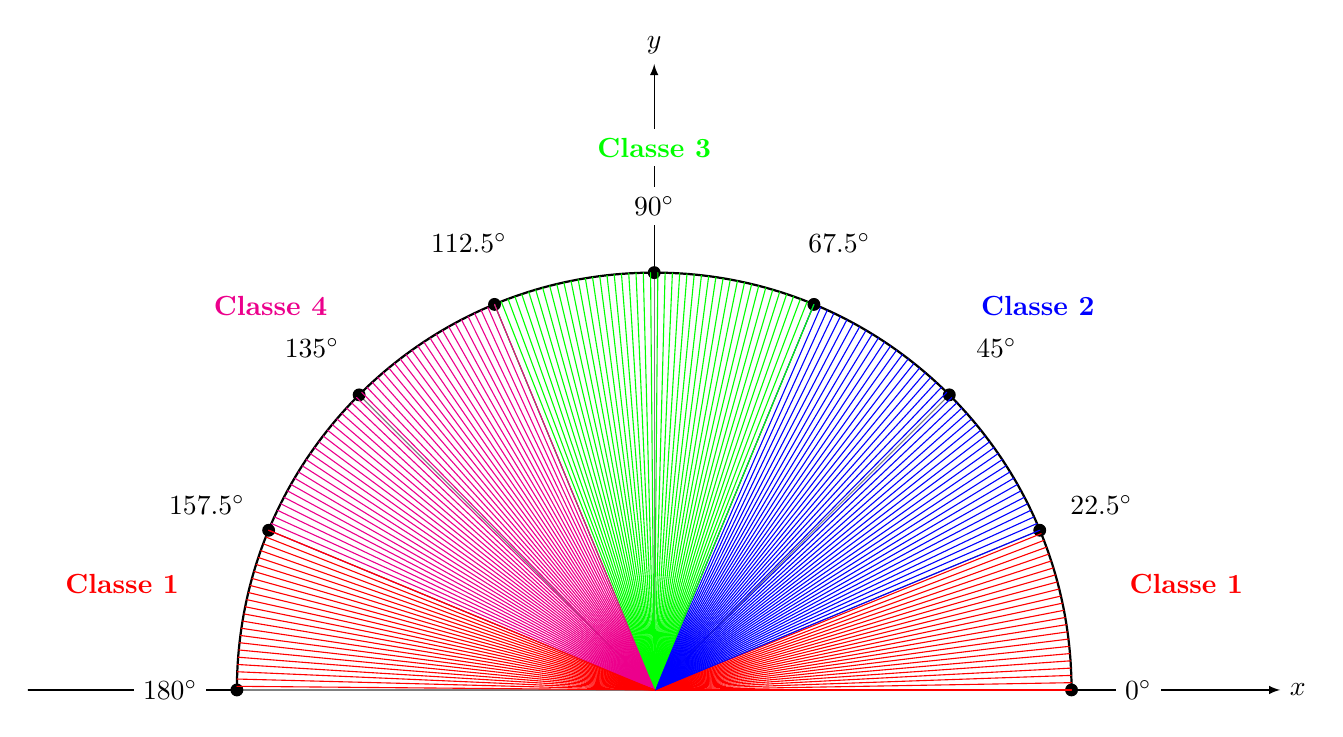
\begin{tikzpicture}[scale=5.3,cap=round,>=latex]
	% draw the coordinates
	\draw[->] (-1.5cm,0cm) -- (1.5cm,0cm) node[right,fill=white] {$x$};
	\draw[->] (0cm,0cm) -- (0cm,1.5cm) node[above,fill=white] {$y$};
	
	% draw the unit circle	
	\begin{scope}
		\clip (-1.5,0) rectangle (1.5,1.5);\clip (-1.5,0) rectangle (1.5,1.5);
		% clip permet d'avoir le demi-cercle
		\draw[thick] (0cm,0cm) circle(1cm);			
	\end{scope}
	
	\foreach \x in {0,22.5,...,180} {
		  % lines from center to point
		  \draw[gray] (0cm,0cm) -- (\x:1cm);
		  % dots at each point
		  \filldraw[black] (\x:1cm) circle(0.4pt);
		  % draw each angle in degrees
		  \draw (\x:1.16cm) node[fill=white] {$\x^\circ$};
	}
	
	\draw (11.25:1.3cm) node[fill=white] {\textcolor{red}{\textbf{Classe 1}}};	
	\draw (45:1.3cm) node[fill=white] {\textcolor{blue}{\textbf{Classe 2}}};
	\draw (90:1.3cm) node[fill=white] {\textcolor{green}{\textbf{Classe 3}}};
	\draw (135:1.3cm) node[fill=white] {\textcolor{magenta}{\textbf{Classe 4}}};
	\draw (168.75:1.3cm) node[fill=white] {\textcolor{red}{\textbf{Classe 1}}};
	
	\foreach \x in {0,1,...,22.5} {
	  % lines from center to point
	  \draw[red] (0cm,0cm) -- (\x:1cm);
	}
	
	\foreach \x in {22.5,23.5,...,67.5} {
	  % lines from center to point
	  \draw[blue] (0cm,0cm) -- (\x:1cm);
	}
	
	\foreach \x in {67.5,68.5,...,112.5} {
	  % lines from center to point
	  \draw[green] (0cm,0cm) -- (\x:1cm);
	}
	  
	\foreach \x in {112.5,113.5,...,157.5} {
	  % lines from center to point
	  \draw[magenta] (0cm,0cm) -- (\x:1cm);
	}
	
	\foreach \x in {157.5,158.5,...,180} {
	  % lines from center to point
	  \draw[red] (0cm,0cm) -- (\x:1cm);
	}
\end{tikzpicture}
\\\\
On traite ensuite les cas suivants : \\
\\
\textcolor{red}{\textbf{Classe 1}} (le contour est dans la direction Nord \--- Sud) : le pixel est un contour si la norme du gradient en ce point est supérieure au maximum de la norme du gradient des pixels Est et Ouest \\
\\
\textcolor{blue}{\textbf{Classe 2}} (le contour est dans la direction Nord-Ouest \--- Sud-Est) : le pixel est un contour si la norme du gradient en ce point est supérieure au maximum de la norme du gradient des pixels Nord-Est et Sud-Ouest \\
\\
\textcolor{green}{\textbf{Classe 3}} (le contour est dans la direction Est \--- Ouest) : le pixel est un contour si la norme du gradient en ce point est supérieure au maximum de la norme du gradient des pixels Nord et Sud \\
\\
\textcolor{magenta}{\textbf{Classe 4}} (le contour est dans la direction Nord-Est \--- Sud-Ouest) : le pixel est un contour si la norme du gradient en ce point est supérieure au maximum de la norme du gradient des pixels Nord-Ouest et Sud-Est \\
\\
Après cette étape, l'image n'est pas encore binarisée mais on a mis à 0 les pixels qui ne constituaient pas un contour.

\subsection{Etape 4/4 : Seuillage par hystérésis}

Le seuillage par hystérésis permet de retirer les faux contours. \\
\\
Pour cela, on définit deux seuils : 
\begin{itemize}
\item[•] \emph{Smin} : seuil minimum
\item[•] \emph{Smax} : seuil maximum \\
\end{itemize}

Pour chaque pixel de la norme du gradient obtenu après la suppression des non-maxima locaux, on regarde sa valeur. \\
\\
\textbf{Cas 1} : si la valeur du pixel est supérieure au seuil maximum alors ce pixel est un vrai contour donc on met sa valeur à 1 \\
\textbf{Cas 2} : si la valeur du pixel est inférieure au seuil minimum alors ce pixel est un faux contour donc on met sa valeur à 0 \\
\textbf{Cas 3} : si la valeur du pixel est entre le seuil minimum et le seuil maximum alors on regarde les valeurs des huit pixels voisins et on regarde s'il existe au moins un pixel voisin qui a une valeur supérieure au seuil maximum. Si c'est le cas, la valeur du pixel initial devient un 1 sinon 0 \\
\\
Pour le \textbf{Cas 3}, dans le code, on prend une fenêtre $3$x$3$ pour obtenir facilement les voisins du pixel au centre de cette fenêtre. \\

\begin{center}
\begin{tikzpicture}[scale=5.3,cap=round,>=latex]
        % draw the coordinates
        \draw (0.75,1.2) node[anchor=south] {\textbf{Vrai contour}};
        \draw[-] (-0.05cm,1cm) -- (1.5cm,1cm) node[right,fill=white] {\emph{Smax}};
        \draw (0.75,0.7) node[anchor=south] {\textbf{Contour incertain}};
        \draw[-] (-0.05cm,0.5cm) -- (1.5cm,0.5cm) node[right,fill=white] {\emph{Smin}};
        \draw (0.75,0.2) node[anchor=south] {\textbf{Faux contour}};
        \draw[-] (0cm,0cm) -- (1.5cm,0cm) node[right,fill=white] {};        
        \draw[->] node[below,fill=none] {$0$} (0cm,0cm) -- (0cm,1.5cm) node[above,fill=white] {$255$} ;
\end{tikzpicture}
\end{center}

L'image obtenue est maintenant binarisée. Elle contient les contours de l'image initiale et un peu de bruit.

\newpage
\section{Bibliographie}
\begin{itemize}

\item[•] \textbf{\textcolor{magenta}{Article}}
\item[\textbf{Titre}] Using Canny's Criteria to Derive a Recursively Implemented Optimal Edge
Detector
\item[\textbf{Auteur}] RACHID DERICHE
\item[]

\item[•] Deriche edge detector
\item[] \url{https://en.wikipedia.org/wiki/Deriche_edge_detector} 

\item[•] Can't get clean output in my MATLAB implementation of Canny-Deriche
\item[] \url{https://stackoverflow.com/questions/14132356/cant-get-clean-output-in-my-matlab-implementation-of-canny-deriche} 

\item[•] Canny edge detector
\item[] \url{https://en.wikipedia.org/wiki/Canny_edge_detector} 

\item[•] Canny Edge Detection Step by step
\item[] \url{https://opencv-python-tutroals.readthedocs.io/en/latest/py_tutorials/py_imgproc/py_canny/py_canny.html} 

\item[•] Détection de contours : les opérateurs de Canny-Deriche
\item[] \url{https://perso.esiee.fr/~coupriem/Algo/algoima.html} 

\item[•] Extraction de contours et son extension du contour actif
\item[]
\url{http://ninebill.free.fr/ExtractionContours/detection/canny.html}

\item[•] JAVA demo of Canny/Deriche-like filter (EPFL Biomedical Imaging Group)
\item[] \url{http://bigwww.epfl.ch/demo/ip/demos/edgeDetector/} 

\item[•] Segmentator \--- Fix gramag export error with deriche filter (3D python)
\item[] \url{https://github.com/ofgulban/segmentator} 

\item[•] Edge Detection with MATLAB
\item[] \url{https://fr.mathworks.com/videos/edge-detection-with-matlab-119353.html} 

\item[•] Gaël Deest (pdf)
\item[] \url{www.theses.fr/2017REN1S102/abes} 

\item[•] Canny en python (OpenCV)
\item[] \url{https://opencv-python-tutroals.readthedocs.io/en/latest/py_tutorials/py_imgproc/py_canny/py_canny.html} 

\item[•] Convolution in Two Dimensions
\item[] \url{http://homepages.inf.ed.ac.uk/rbf/CVonline/LOCAL_COPIES/MARBLE/low/space/convol.htm} 

\item[•] Convolution en 2D
\item[] \url{http://web.stanford.edu/group/sequoia/cgi-bin/node/185} 

\item[•] EECS 442 \--- Computer vision
\item[] \url{http://vhosts.eecs.umich.edu/vision//teaching/EECS442_2012/lectures/lecture14.pdf} 

\item[•] DETECTION DE CONTOURS
\item[] \url{http://www.lirmm.fr/~strauss/PageImage3/EdgeDetection.pdf}

\item[•] Techniques d’extraction de contours
\item[] \url{ftp://ftp-sop.inria.fr/athena/Team/Rachid.Deriche/Lectures/Master-Stic-IGMMV/techniques_contours.pdf}

\item[•] Détection de contours
\item[] \url{http://devernay.free.fr/cours/vision/pdf/c3.pdf}

\item[•] Bases du traitement des images - Détection de contours
\item[] \url{http://webia.lip6.fr/~thomen/Teaching/BIMA/cours/contours.pdf}

\item[•] La détection decontours dans des images à niveaux de gris : mise en œuvre et sélection de détecteurs 
\item[] \url{http://docnum.univ-lorraine.fr/public/INPL_T_1991_ZIOU_D.pdf}

\item[•] Detection de contours
\item[] \url{http://dept-info.labri.fr/~achille/enseignement/TI/TI-ch4-notes.pdf}

\item[•] Segmentation d'image : Contours
\item[] \url{http://www.lgi2p.mines-ales.fr/~montesin/CoursPDF/segmentation_contours.pdf}

\item[•] Filtre de Deriche
\item[] \url{http://www.tsi.enst.fr/pages/enseignement/ressources/mti/Shen_ou_Deriche/node4.html}

\end{itemize}


\end{document}

